% 第三章正文，直接编辑本文件。
\FloatBarrier\clearpage

\section{作品测试与分析}\label{chapter:3}

本章对破茧系统的功能、分析效果、运行性能与安全性进行测试，重点评价浏览记录、观点与论据识别、个人历史比较及长期接触模式分析的准确性，并验证可信执行环境中的数据保护机制。测试既检查浏览作品能否被正确记录，也检查观点与论据能否回到已观察证据、历史比较是否遵循事件时间、持续接触模式是否得到合理解释，以及个人数据是否在授权的可信边界内处理。评价对象为系统在明确观察范围内的工程行为与分析能力，不将内容接触解释为用户认同，不以单一主题集中或内容焦虑表达代替信息茧房及个人心理状态判断。

\subsection{测试目标与总体方案}\label{section:3.1}

\subsubsection{测试目标}\label{section:3.1.1}

测试覆盖内容采集、语义分析、历史检索、状态维护和报告展示等环节。采集层验证作品身份、观看事件和观察片段的区分，避免将采样次数当作作品数量；语义层验证对象条件化的跨模态对齐、主体归属、论证结构和证据定位；历史层验证双路检索、联合覆盖和五维增量；时序层验证低增量重复的持续性及与正常专题学习的区分；安全层验证证明绑定、密钥释放、加密消息与历史检查点；报告层验证统计守恒、未知状态、证据追溯与用户更正。

验收采用功能约束和统计指标相结合的方法。用户隔离、事件幂等、历史时间边界和无效证明拒绝属于必须满足的工程约束；作品识别、论证抽取和接触模式识别使用精确率、召回率、F1 及校准误差评价。各项指标仅对其有效输入范围作出结论，未观察区域及不具备分析依据的样本分别列示。

\subsubsection{测试范围与方法}\label{section:3.1.2}

\begin{longtable}[]{@{}
  >{\RaggedRight\arraybackslash}p{(\linewidth - 8\tabcolsep) * \real{0.1600}}
  >{\RaggedRight\arraybackslash}p{(\linewidth - 8\tabcolsep) * \real{0.2500}}
  >{\RaggedRight\arraybackslash}p{(\linewidth - 8\tabcolsep) * \real{0.2500}}
  >{\RaggedRight\arraybackslash}p{(\linewidth - 8\tabcolsep) * \real{0.2500}}
  >{\RaggedRight\arraybackslash}p{(\linewidth - 8\tabcolsep) * \real{0.0900}}@{}}
\caption{测试范围、目标与评价指标}\label{tab:3-1}\tabularnewline
\toprule\noalign{}
测试模块 & 测试对象及主要输入 & 预期行为 & 主要评价指标 & 结果状态 \\
\midrule\noalign{}
\endfirsthead
\toprule\noalign{}
测试模块 & 测试对象及主要输入 & 预期行为 & 主要评价指标 & 结果状态 \\
\midrule\noalign{}
\endhead
\bottomrule\noalign{}
\endlastfoot
内容对象、事件、语义结果 & 同作品多次打开及同事件多版本 & 三类标识独立，修订不新增观看事件 & 身份一致性、修订一致性 & 通过 \\
增量采集 & 页面变化、图文翻页、关键帧、字幕及音频片段 & 只处理授权可见片段，标记缺口 & 作品计数 P/R、采样去重、覆盖率 & 达标 \\
阅读投入估计 & 正文与评论共屏、滚动、触控、未定位区间 & 时间分配守恒，弱线索不等于实际阅读 & 可见区间 MAE、分配误差、未定位率 & 达标 \\
联合论证理解 & 文字、图像与音频观察版本 & 正确归属主体、条件和论据，输出可定位证据 & 字段 macro-F1、主体准确率、证据定位 & 达标 \\
个人历史增量 & 当前论证及严格过去的多条历史 & 区分复述与新增事实、论据、条件、解释、行动 & Recall@50、五维 macro-F1、联合覆盖 F1 & 达标 \\
时序论证图 & 多日事件、异构关系、缺失掩码及阅读权重 & 识别接触模式，避免专题学习误报 & macro-F1、误报率、ECE & 达标 \\
机密计算 & 证明、报文、加密对象、检查点与删除事务 & 未经放行不释放密钥，拒绝篡改和旧状态 & 拒绝率、状态一致性、恢复开销 & 通过 \\
情绪联合建模 & 情绪---原因候选对、角色及自愿反馈 & 分开呈现内容表达与个人反馈 & 配对 F1、角色 F1、有序误差 & 达标 \\
异步分析 & 突发输入、迟到事件、超时、重连 & 阶段结果可用、队列稳定、最终一致 & 接收 P95、完成 P95、积压及恢复时间 & 达标 \\
聚合展示 & 小时、自然日、滚动窗口及多设备重叠 & 分母明确、时间守恒、证据可回看 & 聚合一致性、追溯完整性 & 通过 \\
\end{longtable}

单元测试验证字段、区间和密码接口；服务测试验证事件状态与授权；端到端测试对照人工操作轨迹；离线模型评价使用隔离测试集；性能测试按固定负载回放；安全测试按协议状态注入异常。训练超参数、判定阈值和置信校准仅使用训练与验证数据，测试集在模型与配置冻结后一次性评价。模型实验使用 3 个随机种子，表中报告均值；置信区间按原始作品或用户整组重采样，而不是按同作品的观察版本独立重采样。

\subsection{测试环境搭建与设备}\label{section:3.2}

\subsubsection{端侧与浏览器环境}\label{section:3.2.1}

手机测试覆盖 OPPO/ColorOS、vivo/OriginOS、小米/HyperOS、荣耀/MagicOS、三星/One UI 及 Pixel/原生 Android 六类终端，每类设置 2 台设备，共 12 台物理设备。测试涵盖 Android 12 至 14、8 至 12 GB 内存及 60 Hz 和 120 Hz 显示模式，重点检查无障碍节点差异、后台运行限制、屏幕采集授权和作品切换时的状态保持。受控测试应用提供可核验的作品标识、固定操作脚本和显示时间；真实平台测试采用授权操作轨迹，平台版本随测试批次固定。Android 模拟器用于异常流程复现，不替代真机前台流畅度与页面识别评价。

浏览器端使用 Chromium 环境，通过具有明确内容标识的受控网页核对 DOM 增量、正文与评论分离、鼠标悬停线索和窗口可见性。手机和浏览器均使用单调时钟测量持续时长，设备时钟用于事件时间与时区归档，服务器接收时间独立记录。网络条件包括稳定 Wi-Fi、蜂窝网络和受控弱网；弱网注入 100 毫秒附加往返时延、1\%丢包及 60 秒断网，分开评价网络开销与服务计算开销。

\subsubsection{云端计算与可信环境}\label{section:3.2.2}

\begin{longtable}[]{@{}
  >{\RaggedRight\arraybackslash}p{(\linewidth - 6\tabcolsep) * \real{0.1600}}
  >{\RaggedRight\arraybackslash}p{(\linewidth - 6\tabcolsep) * \real{0.2800}}
  >{\RaggedRight\arraybackslash}p{(\linewidth - 6\tabcolsep) * \real{0.2800}}
  >{\RaggedRight\arraybackslash}p{(\linewidth - 6\tabcolsep) * \real{0.2800}}@{}}
\caption{云端测试设备与用途}\label{tab:3-2}\tabularnewline
\toprule\noalign{}
环境 & 公开云实例及配置 & 使用范围 & 可信边界 \\
\midrule\noalign{}
\endfirsthead
\toprule\noalign{}
环境 & 公开云实例及配置 & 使用范围 & 可信边界 \\
\midrule\noalign{}
\endhead
\bottomrule\noalign{}
\endlastfoot
普通 GPU 环境 & AWS EC2 g5.2xlarge；8 vCPU、32 GiB 内存、1 张 NVIDIA A10G，产品页标称 24 GB GPU 内存 & 脱敏数据基线、负载发生与轻量组件对照 & 不作为本项目机密 GPU 证明环境 \\
CPU 机密环境 & Azure Standard\_\allowbreak{}DC8as\_\allowbreak{}v5；8 vCPU、32 GiB 内存、AMD SEV-SNP，无 GPU & CPU 可信处理、检索、状态事务及协议验证 & 客体操作系统与获准服务属于可信计算基 \\
GPU 机密环境 & Azure Standard\_\allowbreak{}NCC40ads\_\allowbreak{}H100\_\allowbreak{}v5；40 vCPU、320 GiB 内存、1 张 H100 NVL，94 GB GPU 内存 & 多模态联合模型、异步推理、真实机密 GPU 测试 & 经验证的 CPU、GPU 及其受保护通信链路 \\
\end{longtable}

测试采用表~\ref{tab:3-2}所列云端环境，普通 GPU 用于基线对照，CPU 机密环境用于受保护检索与状态事务，机密 GPU 环境用于多模态推理及性能评价。

\begin{longtable}[]{@{}
  >{\RaggedRight\arraybackslash}p{(\linewidth - 4\tabcolsep) * \real{0.2000}}
  >{\RaggedRight\arraybackslash}p{(\linewidth - 4\tabcolsep) * \real{0.4000}}
  >{\RaggedRight\arraybackslash}p{(\linewidth - 4\tabcolsep) * \real{0.4000}}@{}}
\caption{软件测试配置}\label{tab:3-3}\tabularnewline
\toprule\noalign{}
组件 & 实验配置 & 用途与约束 \\
\midrule\noalign{}
\endfirsthead
\toprule\noalign{}
组件 & 实验配置 & 用途与约束 \\
\midrule\noalign{}
\endhead
\bottomrule\noalign{}
\endlastfoot
客体系统 & Ubuntu 22.04 LTS，机密实例使用厂商兼容镜像 & 常规/机密对照分别记录镜像摘要 \\
Python 与训练 & Python 3.11、PyTorch 2.5、CUDA 12.4 兼容运行时 & LoRA、任务头训练和推理 \\
OCR 与 ASR & PaddleOCR 2.9、Whisper large-v3-turbo & 固定识别器权重与预处理配置 \\
移动客户端 & Kotlin、Android SDK 34、Compose、Room & 事件、区间与版本管理 \\
密码与证明 & OpenSSL 3.0 系列、厂商证明 SDK & 固定安全补丁与验证材料，不自行实现密码原语 \\
浏览器 & Chromium 128 兼容测试环境 & 受控 DOM、可见性与交互轨迹 \\
\end{longtable}

各组实验采用一致的软件版本、模型权重与预处理配置。服务采用 Linux 客体系统，固定组件和模型版本。镜像、模型权重、提示模板、工具权限和分析配置组成版本清单，加载器验证摘要后锁定会话版本。日志只保留不透明任务编号、阶段状态及资源指标，原文、向量和诊断详情保存在用户授权的受保护对象内。

协议联调使用明确标识的 Mock 证明；CPU 与 GPU 机密执行使用硬件证明和相应验证链。GPU 配置核验参考 Azure 机密 GPU 说明\cite{ref33}。只有 CPU 隔离不能证明 GPU 张量及设备内存受到相同保护，普通 GPU 结果不计入机密 GPU 安全结论。

\subsubsection{实验控制与测量方法}\label{section:3.2.3}

模型评价固定输入版本和观察范围。精细理解采用不超过 2,048 个文本 token、最多 8 张关键帧及 30 秒已授权音频片段的单任务上限，长视频按片段处理并保留关联。训练在 GPU 环境中使用 LoRA 及任务头联合学习，公共语料仅承担其已具备字段的迁移监督，中文目标域负责本项目字段与置信校准。任务掩码跳过缺失标签，不将未标注字段作为负例。

性能测试固定 50\%纯文字、30\%图文和 20\%视频片段的事件混合比例，每事件平均触发 1 次初步理解、0.5 次 OCR、0.2 次 ASR、0.3 次跨模态精细理解、1 次历史比较及 1 次图更新。批处理上限为 8，模型和版本策略固定，比较机密与常规执行时使用相同硬件规格及输入序列。A10G 与 H100 跨硬件差异不用于推导机密计算开销。

\subsection{测试数据与标注规范}\label{section:3.3}

\subsubsection{数据集构成}\label{section:3.3.1}

\begin{longtable}[]{@{}
  >{\RaggedRight\arraybackslash}p{(\linewidth - 6\tabcolsep) * \real{0.2500}}
  >{\RaggedRight\arraybackslash}p{(\linewidth - 6\tabcolsep) * \real{0.2500}}
  >{\RaggedRight\arraybackslash}p{(\linewidth - 6\tabcolsep) * \real{0.2500}}
  >{\RaggedRight\arraybackslash}p{(\linewidth - 6\tabcolsep) * \real{0.2500}}@{}}
\caption{自建数据集及评价用途}\label{tab:3-4}\tabularnewline
\toprule\noalign{}
数据集 & 规模与组成 & 核心标注 & 评价用途 \\
\midrule\noalign{}
\endfirsthead
\toprule\noalign{}
数据集 & 规模与组成 & 核心标注 & 评价用途 \\
\midrule\noalign{}
\endhead
\bottomrule\noalign{}
\endlastfoot
跨平台多模态作品与论证 & 6,000 个作品；小红书图文、小红书短视频、抖音短视频各 2,000 个；每作品 3 个观察版本，共 18,000 个版本 & 对象、主体、观点短语、立场、条件、论据、引用/反驳及证据索引 & 多模态理解与部分观察修订 \\
个人历史信息增量 & 12,000 组当前材料---过去历史样本，每组允许多条历史 & 五维增量、联合覆盖、同源关系、证据不足 & 检索、关系判断与信息增量 \\
长期接触序列 & 200 名自愿参与者，每人 14 天，共 2,800 个用户日 & 有效观察、接触模式、阅读目的、回顾依据 & 时序图、校准及长期解释 \\
情绪---原因---角色 & 8,000 个上下文片段，来自上述作品 & 情绪与原因跨度、持有者、对象、归属、认知评价、处境、表达方式 & 联合情绪模型及反馈分离 \\
页面与安全回归 & 240 条操作轨迹，两平台各 120 条；120 个协议与状态场景 & 真实作品边界、可见区间、状态转移及拒绝条件 & 计数、停留估计及安全一致性 \\
\end{longtable}

作品采样覆盖就业与教育、性别与家庭、科技与产品、经济与消费、健康与生活、公共议题六类领域，每类 1,000 个作品。领域用于采样分层，实际观点使用``当前招聘困难''\,``职业能力需要持续提升''等可回到原文的短语，并保留对象、时态和条件，不将``经济与消费''等领域名称作为观点结论。

数据记录包括平台内标识、匿名作者标识、时间、可见正文、授权媒体、OCR/ASR 片段、评论线程及覆盖范围。授权按参与者、应用和媒体类型分别管理，授权撤回与删除操作均进入测试流程；私人聊天、未授权后台内容与隐藏页面不进入语料。数据获取不绕过平台权限和访问限制，身份映射与分析材料分开保存。模型训练使用经过单独授权和脱敏处理的材料，不将参与者全部个人历史默认用于训练。

样本来源、授权范围和撤回状态分别记录，数据使用限定在参与者同意的研究范围内。

\subsubsection{数据划分与泄漏防范}\label{section:3.3.2}

原始作品按作者、作品身份及同源近重复组统一划分，训练/验证/测试分别为 4,200/900/900 个作品，相应观察版本为 12,600/2,700/2,700 个。依赖作品的增量样本和情绪样本继承同一划分：增量样本为 8,400/1,800/1,800 组，情绪片段为 5,600/1,200/1,200 条。分层组分配在构建样本之前完成，跨组依赖样本不纳入本轮划分；同一作品的早期与完整版本不会分别进入训练和测试。

测试集作品在六个领域各 150 个，三种平台/媒体组合各 300 个。增量测试集覆盖八类情形，每类 225 组，共 1,800 组：同观点新论据、同义改写重复、条件扩展、解释变化、行动变化、引用后反驳、同源转载和证据不足。这些情形用于分层抽样而非互斥的五维增量标签，一个样本可以同时包含多种增量。

长期评价设置两套独立协议。用户隔离协议采用 140/30/30 名用户，分别对应 1,960/420/420 个用户日；测试用户的个性化反馈不能用于训练。时间隔离协议在全部 200 名用户内按前 8 天、随后 3 天、最后 3 天划分，分别为 1,600/600/600 个用户日，只有早期反馈参与个体适配。两套协议的结果分别报告，不相加为独立样本总量。测试期历史可作为当时已观察上下文，但其测试标签不参与参数更新或调阈值。

用户日表示安排的观察单位，不代表全天完整采集。缺失区间按原因和持续时间保存，没有观测的日期标为缺失。历史比较对每次当前观察采用严格小于该观察时点的材料，并读取当时已可用版本；后续补充、未来评论及后来取得的完整视频不进入早期历史判断。

\subsubsection{标注与一致性}\label{section:3.3.3}

语义样本由两名标注者独立标注，第三人裁决分歧。观点、立场和条件标签一致性使用 Cohen's κ，论证与情绪跨度使用标注者间 F1，有序评价使用加权κ。实验中立场κ为 0.84，增量标签平均κ为 0.79，论证证据跨度 F1 为 0.88，情绪---原因配对 F1 为 0.85，有序认知评价加权κ为 0.76。裁决后保留争议类型及支持片段，而不将一致性数值解释为标注完全正确。

认知评价采用目标受阻、威胁或损失、结果不确定性、自身控制可能、应对资源五个维度。每维使用五级强度，缺乏材料或未提及单独记录适用性。内容人物的表达、引述人物的表达与参与者自报分别标注，不能用页面停留时间自动生成个人情绪标签。

\subsection{功能、采集与统计一致性测试}\label{section:3.4}

\subsubsection{作品计数及可见停留}\label{section:3.4.1}

240 条轨迹共包含 2,920 次进入作品的观看事件。对每条轨迹按平台和人工核验作品标识去重后，累计为 2,540 个轨迹内作品；同作品再次打开增加观看事件，不增加该轨迹内去重作品数。单次观看中的文案展开、图像翻页和评论开关增加片段或修订，不增加作品数。

计数识别输出 2,900 次候选事件，与人工边界匹配得到 TP=2,856、FP=44、FN=64，精确率为 98.48\%，召回率为 97.81\%，F1 为 98.14\%，达到两项均不低于 95\%的验收要求。匹配使用作品身份和时间重叠联合约束，每个预测与真值至多匹配一次。错误集中在极快切换、遮挡过渡与平台页面结构变化，说明系统减少了重复计数，但未达到任意页面下完全不重不漏。

按区间端点计算的可见停留 MAE 为 1.12 秒，P95 绝对误差为 2.80 秒；验收约束作用于 MAE 而非所有样本最大误差。正文与评论阅读投入以人工回顾定位作为参考，平均时长绝对误差为 1.65 秒，未定位时长占有效观察时长的 8.6\%。该项衡量估计与参考的一致性，不等同于眼动测量或认知投入真值。

\subsubsection{状态、恢复与报告验证}\label{section:3.4.2}

\begin{longtable}[]{@{}
  >{\RaggedRight\arraybackslash}p{(\linewidth - 10\tabcolsep) * \real{0.0800}}
  >{\RaggedRight\arraybackslash}p{(\linewidth - 10\tabcolsep) * \real{0.1300}}
  >{\RaggedRight\arraybackslash}p{(\linewidth - 10\tabcolsep) * \real{0.2200}}
  >{\RaggedRight\arraybackslash}p{(\linewidth - 10\tabcolsep) * \real{0.2300}}
  >{\RaggedRight\arraybackslash}p{(\linewidth - 10\tabcolsep) * \real{0.2600}}
  >{\RaggedRight\arraybackslash}p{(\linewidth - 10\tabcolsep) * \real{0.0800}}@{}}
\caption{功能及一致性用例}\label{tab:3-5}\tabularnewline
\toprule\noalign{}
用例编号 & 测试对象 & 输入或步骤 & 预期结果 & 评价指标与结果 & 状态 \\
\midrule\noalign{}
\endfirsthead
\toprule\noalign{}
用例编号 & 测试对象 & 输入或步骤 & 预期结果 & 评价指标与结果 & 状态 \\
\midrule\noalign{}
\endhead
\bottomrule\noalign{}
\endlastfoot
TC-01 & 同作品增量 & 翻页、字幕新增、文案展开及评论开关 & 原事件修订，作品身份稳定 & 与人工计数联合核验，P=98.48\%、R=97.81\% & 达标 \\
TC-02 & 事件幂等 & 相同事件与修订重复发送，重复与并发混合 & 返回已有状态，统计贡献一次 & 10,000 次提交的贡献一致性 100\% & 通过 \\
TC-03 & 修订替换 & 修改观点或补充媒体片段 & 先撤销旧贡献再应用新贡献 & 1,000 组序列无重复贡献 & 通过 \\
TC-04 & 迟到及时间边界 & 断网补传、乱序、未来版本与同时间事件 & 严格过去历史，重算受影响范围 & 600 组时间用例全部符合预期 & 通过 \\
TC-05 & 中断恢复 & 阶段任务重启与 60 秒断网 & 重试不新增事件，阶段可恢复 & 300 次恢复后版本及摘要一致 & 通过 \\
TC-06 & 多用户隔离 & 相同标识、不同凭据，跨用户检索和删除 & 拒绝越权，缓存和记忆隔离 & 500 组隔离请求无跨用户对象返回 & 通过 \\
TC-07 & 多设备重叠 & 两设备同时间浏览与跨小时事件 & 单设备分别展示，个人时间取并集 & 500 组区间用例守恒 & 通过 \\
TC-08 & 时区聚合 & 自然日、滚动 24 小时、7 天及夏令时切换 & 真实时长按时区偏移分桶 & 240 组窗口用例分子分母一致 & 通过 \\
TC-09 & 证据回看 & 点击小时、观点及历史关系 & 返回对应修订与原文/媒体位置 & 900 个测试作品的索引结构完整 & 通过 \\
TC-10 & 用户更正及删除 & 修改归属、删除原事件及派生依赖 & 新报告不引用已删除对象 & 300 组依赖重算与报告检查通过 & 通过 \\
\end{longtable}

上述功能用例与 240 条轨迹及 120 个安全场景是不同计数单位：功能用例由场景参数化生成，不另充当自然作品或独立模型样本。工程约束用例全部通过只说明约定输入满足规则，不代表语义模型准确率为 100\%。

日报按自然日展示，过去 24 小时按查询截止点回溯，最近 7 天同时标明观察有效日数。未知观点、证据不足、等待处理与采集失败分别统计。观点采用多标签，比例以同一窗口内可分析去重作品为分母，允许合计超过 100\%；未知作品另列，不把多标签比例画成互斥饼图。需要饼图时仅展示主观点分配，并显式保留混合及未定位类别。

\subsubsection{同一作品多片段的端到端验证}\label{section:3.4.3}

本项测试验证页面变化是否被错误当成作品切换。小红书图文作品 W-A 的观看事件 E-A 于 10:59:42 开始、11:00:18 结束，共 36 秒。操作依次为阅读正文 12 秒、翻阅图片 8 秒、打开评论 10 秒、返回正文 6 秒。系统生成 4 次内容修订，保持作品数 1、观看次数 1，正文与图片分配 26 秒、评论 10 秒，合计不超过可见区间。案例内容依据本章数据集设定构造，不冒充真实个人记录或平台截图。

作品讨论``就业需要结合行业差异''。正文写有``不同岗位不能一概而论''，第二张图提供行业分组，评论中出现被反驳的``所有行业都没有机会''。理解模块保留作者观点、图片论据及评论引用/反驳关系，不把评论表达归给正文作者。图片翻页使论据由未定位修订为已定位，不产生新作品。

小时聚合分别计入 10 时段 18 秒和 11 时段 18 秒，两小时各包含 1 个作品，但日去重作品仍为 1。小时作品数不能简单相加为日作品数；跨小时的同一事件在详情中明确标识。点击任一小时能够回看同一事件及对应片段，修订替换旧贡献而不重复累加。

\begin{figure}[htbp]
\centering
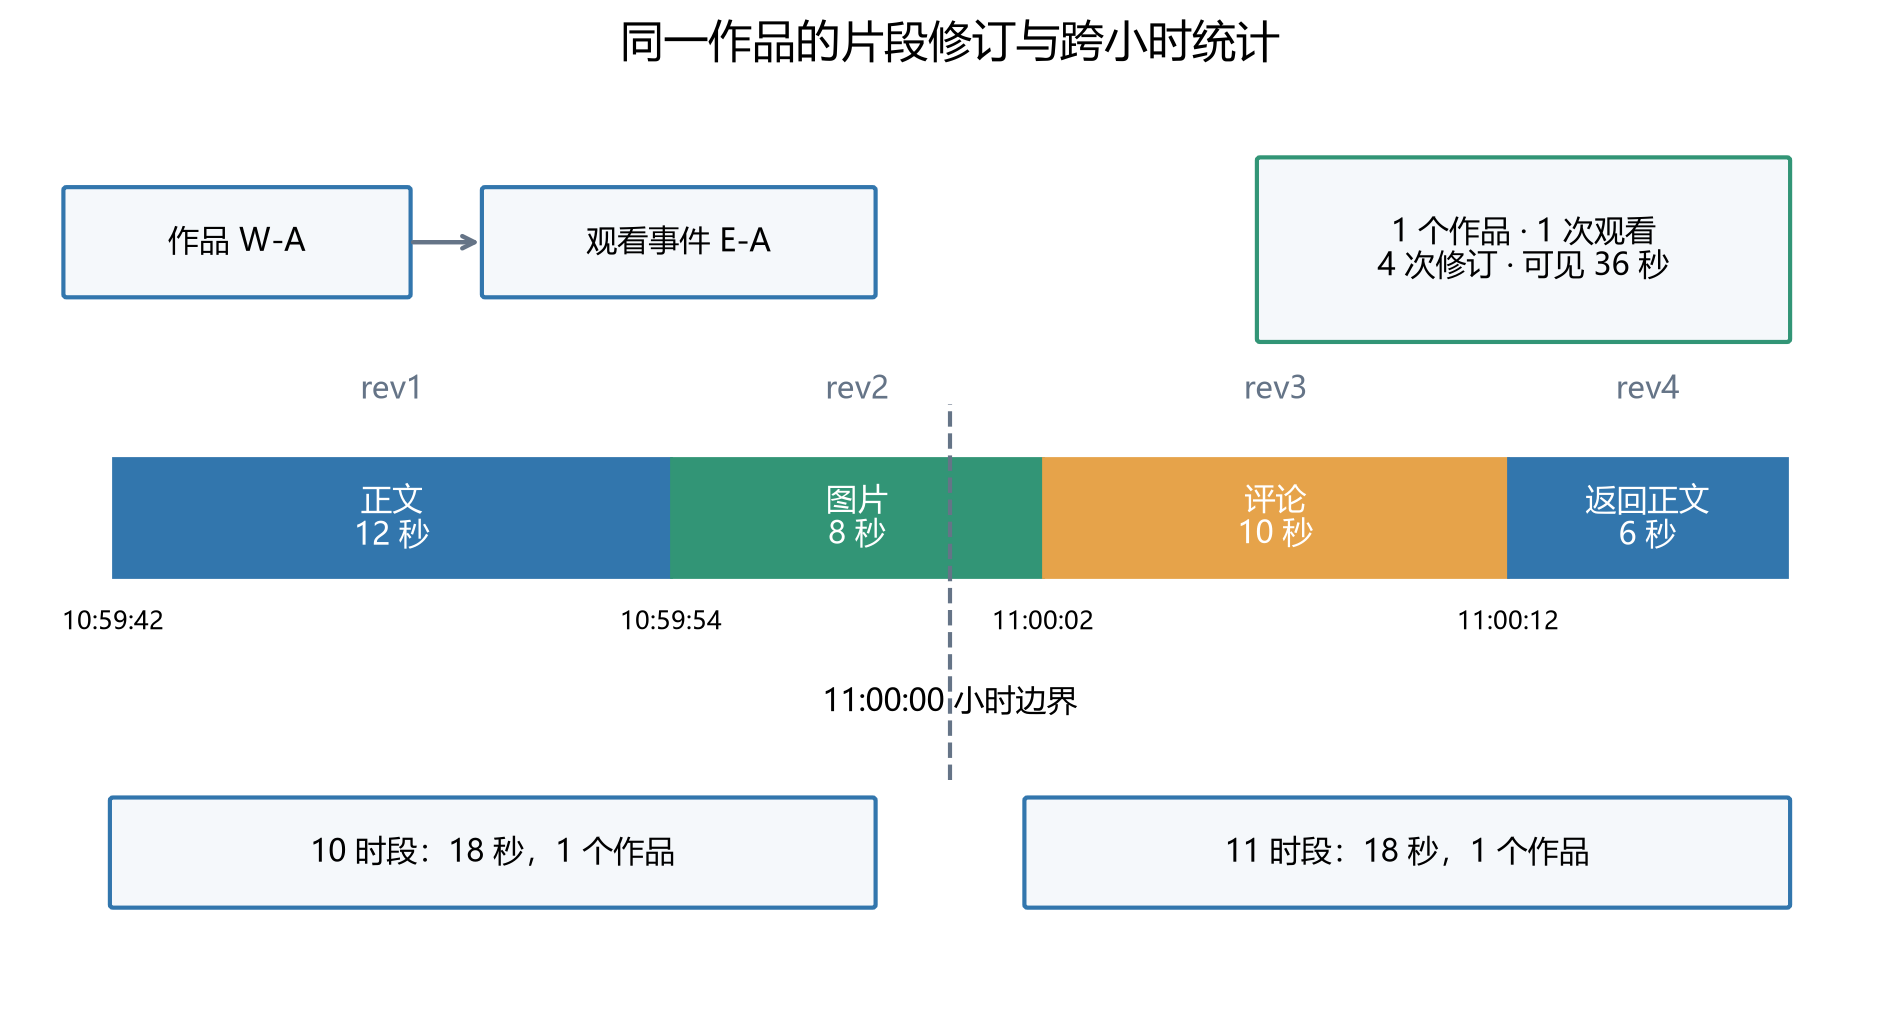
\includegraphics[width=\linewidth,height=0.66\textheight,keepaspectratio]{figures/chapter3/图3-1.png}
\caption{同一作品的片段修订与跨小时统计}\label{fig:3-1}
\end{figure}

\begin{figure}[htbp]
\centering
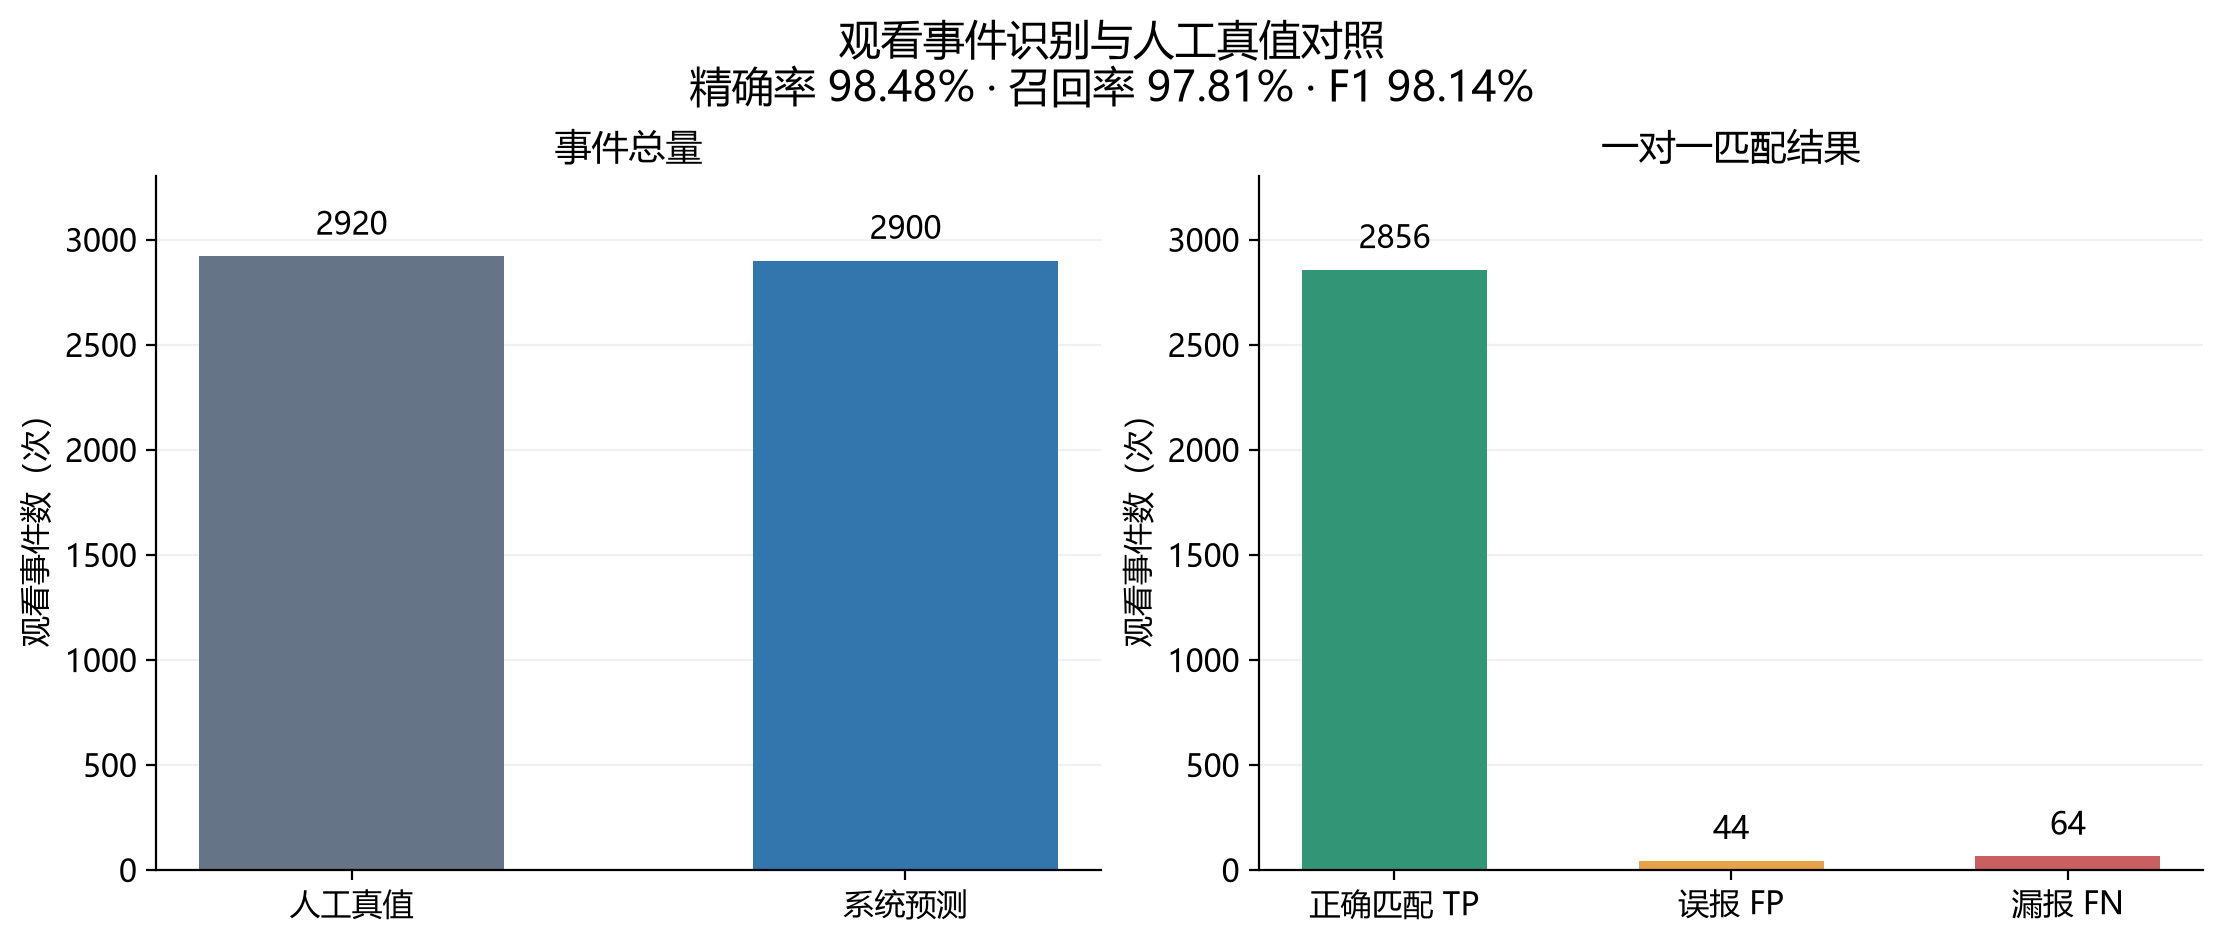
\includegraphics[width=\linewidth,height=0.66\textheight,keepaspectratio]{figures/chapter3/图3-2.png}
\caption{观看事件识别与人工真值对照}\label{fig:3-2}
\end{figure}

\subsubsection{相近观点与不同论据的端到端验证}\label{section:3.4.4}

第二个案例检验相同观点是否掩盖新增依据。用户在 09:10、09:18 及 10:05 依次接触 W-B/C/D，均围绕``当前招聘困难''。展示短语之外保留对象、时态、条件和论据，主题相似并非完全可比的充分条件。

W-B 正文呈现``某行业本月招聘岗位减少''，配图限定某城市应届岗位。W-C 字幕转述相同数据，画面显示同一匿名统计出处。双路检索召回 W-B，交叉判别确认范围相容，联合覆盖命中旧数据。W-C 与 W-B 归入同一观点并建立论据复用关系，但仍是两个实际浏览作品，不能因观点相同删除作品计数。

W-D 增加``部分岗位提高经验门槛''的材料，补充另一个行业条件及``区分岗位类型再投递''的建议。五维结果为事实新增、论据新增、条件新增、解释待定、行动新增。因片段不足以说明门槛变化的因果机制，解释维度保持待定。新增数据不自动转化为新增因果解释。

三条材料按同一观点展示时，作品数为 3、观点组为 1；其中 W-B 为首份材料，W-C 复用旧论据，W-D 包含新增依据。小时详情分别链接正文、关键帧或音频位置及过去历史。在 7 天案例序列中，20 个可分析作品有 16 个表达相近观点，占 80\%；其中 6 个包含新增论据，10 个为低增量重复。长期解释结合持续性、来源关系和阅读目的，不根据 80\%的集中度单独断言信息茧房。

\begin{figure}[htbp]
\centering
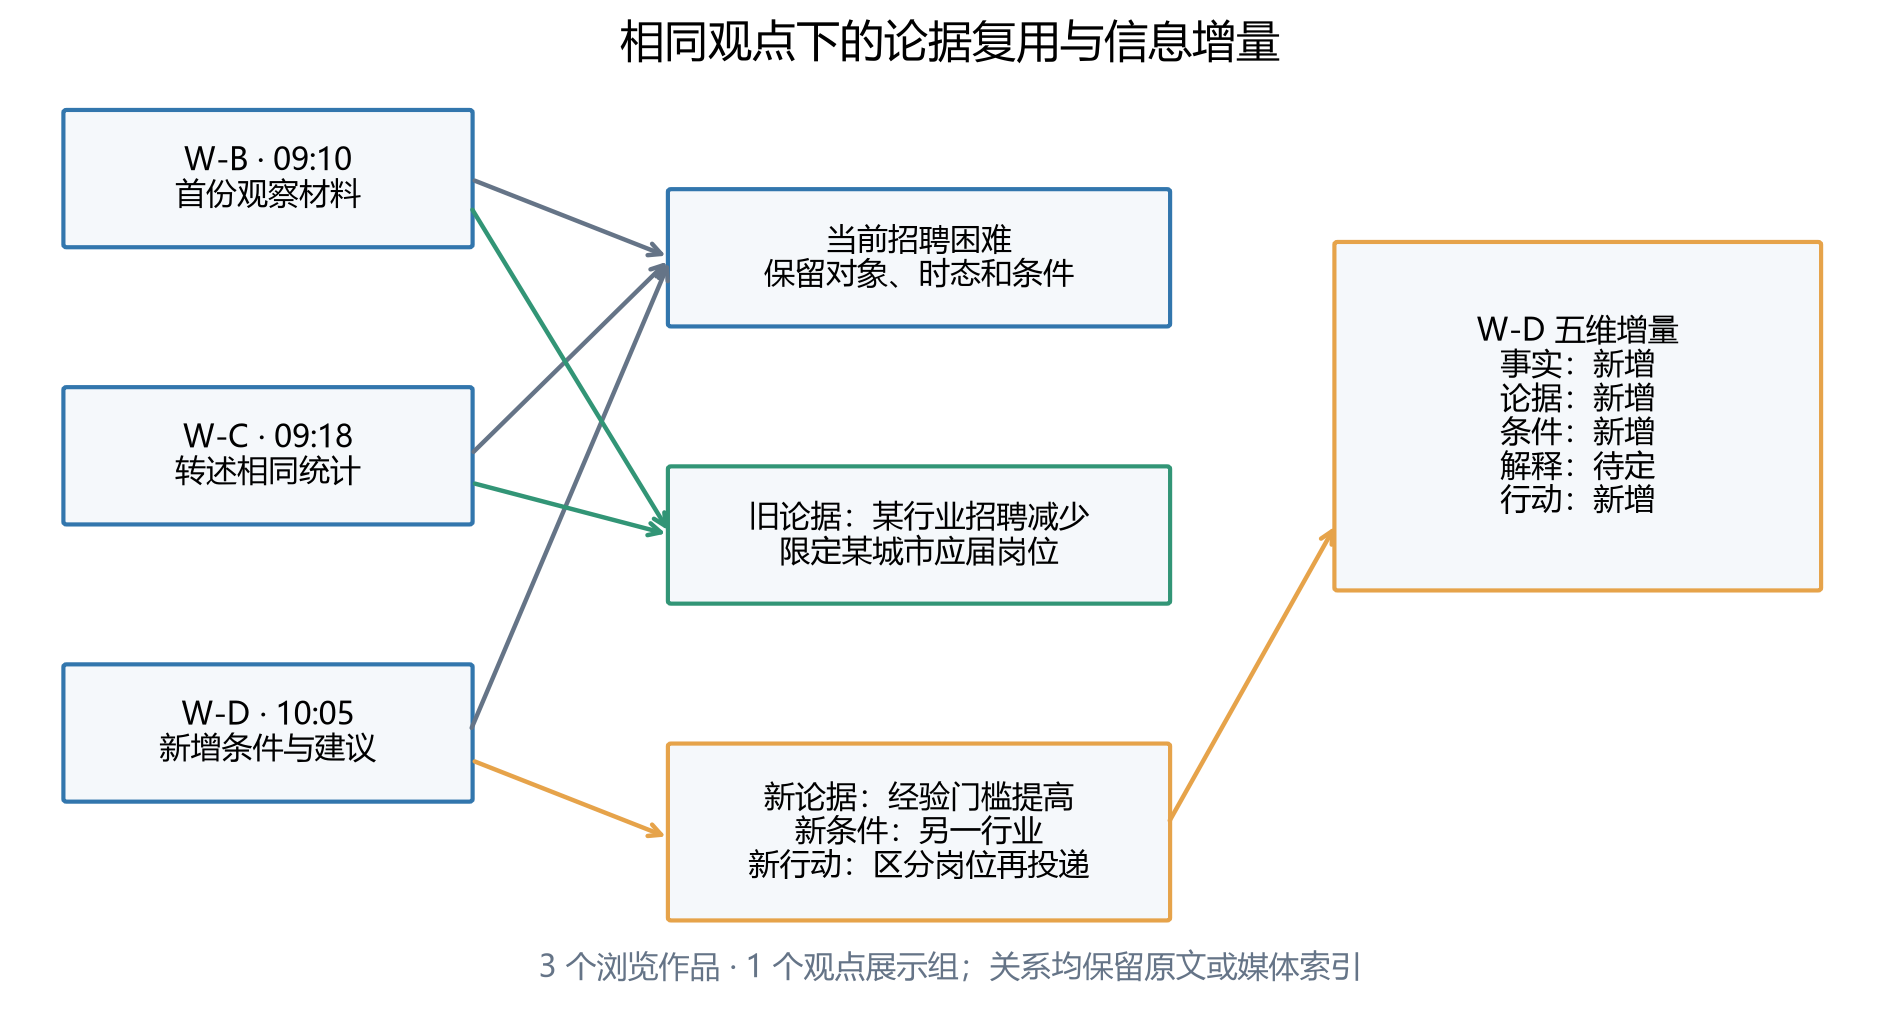
\includegraphics[width=\linewidth,height=0.66\textheight,keepaspectratio]{figures/chapter3/图3-3.png}
\caption{相同观点下的论据复用与信息增量}\label{fig:3-3}
\end{figure}

\subsection{多模态论证与个人历史增量评价}\label{section:3.5}

\subsubsection{论证联合理解}\label{section:3.5.1}

论证字段 macro-F1 分别计算主张、对象、立场、条件、论据与关系，再进行等权平均。实体跨度采用精确匹配，并另报告证据位置容差指标；主体归属在可判定样本上计算准确率，不用拒识样本扩大正确数。拒识覆盖率和已接受样本错误率共同报告。

\begin{longtable}[]{@{}
  >{\RaggedRight\arraybackslash}p{(\linewidth - 8\tabcolsep) * \real{0.1800}}
  >{\RaggedRight\arraybackslash}p{(\linewidth - 8\tabcolsep) * \real{0.2000}}
  >{\RaggedRight\arraybackslash}p{(\linewidth - 8\tabcolsep) * \real{0.2000}}
  >{\RaggedRight\arraybackslash}p{(\linewidth - 8\tabcolsep) * \real{0.2200}}
  >{\RaggedRight\arraybackslash}p{(\linewidth - 8\tabcolsep) * \real{0.2000}}@{}}
\caption{论证模型及消融结果}\label{tab:3-6}\tabularnewline
\toprule\noalign{}
方法 & 字段 macro-F1 & 主体归属准确率 & 证据定位 F1 & 已接受样本错误率 \\
\midrule\noalign{}
\endfirsthead
\toprule\noalign{}
方法 & 字段 macro-F1 & 主体归属准确率 & 证据定位 F1 & 已接受样本错误率 \\
\midrule\noalign{}
\endhead
\bottomrule\noalign{}
\endlastfoot
纯文字理解 & 0.752 & 0.854 & 0.731 & 12.8\% \\
文本、图像、音频直接拼接 & 0.787 & 0.881 & 0.768 & 11.3\% \\
移除对象条件化对齐 & 0.814 & 0.902 & 0.801 & 9.4\% \\
移除质量门控 & 0.819 & 0.910 & 0.805 & 10.6\% \\
移除证据定位监督 & 0.811 & 0.906 & 0.763 & 9.8\% \\
完整联合模型 & 0.846 & 0.934 & 0.862 & 7.1\% \\
\end{longtable}

完整模型字段 macro-F1 的 95\%整组自助法置信区间为{[}0.832,0.860{]}，主体归属准确率为{[}0.920,0.947{]}，均达到内部验收要求。已接受样本覆盖率为 88.4\%，其余保留证据不足或冲突状态；不能用仅接受高置信样本的指标代表全部输入准确率。

早期、中期、完整观察版本的字段 macro-F1 分别为 0.718、0.791 和 0.846。新增片段通过修订提高可判定程度，而没有把完整作品中的信息回填为早期已经观察的事实。跨模态对齐改善图中说明与语音转述的对象归属，质量门控主要减少低清图像和噪声音频引入的错误。残余错误包括反讽、多个主体同屏、隐含条件及 OCR 误识别。

\subsubsection{历史召回、关系判别与联合覆盖}\label{section:3.5.2}

历史评价先检索再判别，Recall@50 按每个当前材料所需的人工标注历史集合计算并宏平均；关系 F1 区分支持、矛盾、引用后反驳、条件变化和不可比状态。五维增量分别评价，不用主题相似度代替增量。

\begin{longtable}[]{@{}
  >{\RaggedRight\arraybackslash}p{(\linewidth - 6\tabcolsep) * \real{0.2500}}
  >{\RaggedRight\arraybackslash}p{(\linewidth - 6\tabcolsep) * \real{0.2500}}
  >{\RaggedRight\arraybackslash}p{(\linewidth - 6\tabcolsep) * \real{0.2500}}
  >{\RaggedRight\arraybackslash}p{(\linewidth - 6\tabcolsep) * \real{0.2500}}@{}}
\caption{历史比较方法对照}\label{tab:3-7}\tabularnewline
\toprule\noalign{}
方法 & Recall@50 & 五维增量 macro-F1 & 联合覆盖 F1 \\
\midrule\noalign{}
\endfirsthead
\toprule\noalign{}
方法 & Recall@50 & 五维增量 macro-F1 & 联合覆盖 F1 \\
\midrule\noalign{}
\endhead
\bottomrule\noalign{}
\endlastfoot
字面匹配与主题过滤 & 0.704 & 0.611 & 0.587 \\
单路语义向量 & 0.853 & 0.744 & 0.718 \\
双路召回、不使用交叉判别 & 0.927 & 0.776 & 0.751 \\
双路与交叉判别、仅单条历史覆盖 & 0.927 & 0.802 & 0.768 \\
完整双路与联合覆盖 & 0.941 & 0.837 & 0.858 \\
\end{longtable}

完整模型五维 F1 分别为事实 0.856、论据 0.872、条件 0.811、解释 0.824、行动 0.822，等权平均为 0.837。召回 Recall@50 为 0.941，达到 0.90 要求；五维 macro-F1 达到 0.80 要求。条件扩展和解释变化仍是主要误差来源，涉及省略语境时系统保留不确定状态。

联合覆盖将当前论据拆为可定位单元，并允许多个历史共同覆盖。完整方法较单条历史方法提高联合覆盖 F1 共 0.090，减少``旧论据分散在不同作品中，因此被当成新内容''的错误。对同观点新论据样本，模型保留观点重复与论据新增两个不同结果；对引用后反驳样本，引用命中不自动生成支持关系。

时间边界压力样本中，未来版本、同时间观察和后来补充的完整媒体均未进入早期历史候选；这是独立的工程约束，不由语义 F1 证明。信息增量只描述相对于已接触材料的新颖程度，不承担外部事实核查职责。

\subsubsection{误差案例与处置}\label{section:3.5.3}

案例一为快速切换中的过渡遮挡。用户在 0.8 秒内从视频 A 滑到 B，过渡帧仅有``关注''\,``评论''等公共控件，作者与标题暂不可见。按全文变化切分的方法会产生第三个作品。完整方法将其保留为未确认片段，取得稳定锚点后归入 B；如果未能取得，则不冒充已确认作品。计数仍有 44 次误报和 64 次漏报，主要说明极快切换与结构变化未完全解决。用户更正会撤销旧贡献并重算，不只修改列表文字。

案例二为引用后反讽。前半句为``大家都说`学历越高越没用'\,''，后半句为``那为什么不少岗位仍设置学历门槛''。早期片段仅有引用时，模型保留主体及立场不确定；后续音频抵达后，将引用归给被转述群体，作者表达修订为质疑。如果字幕漏识别否定词，质量门控保留模态冲突，不用一个模态的高置信掩盖冲突。该例展示迟到修订，不能替代测试集准确率。

案例三为隐含条件。相同``招聘困难''表达分别讨论应届生与有经验者，条件被截断时容易误判完全重复。补充片段后分别保存条件，撤销早期关系及其统计贡献，重放受影响图记忆；观察不足时不输出确定的零增量判断。

\begin{figure}[htbp]
\centering
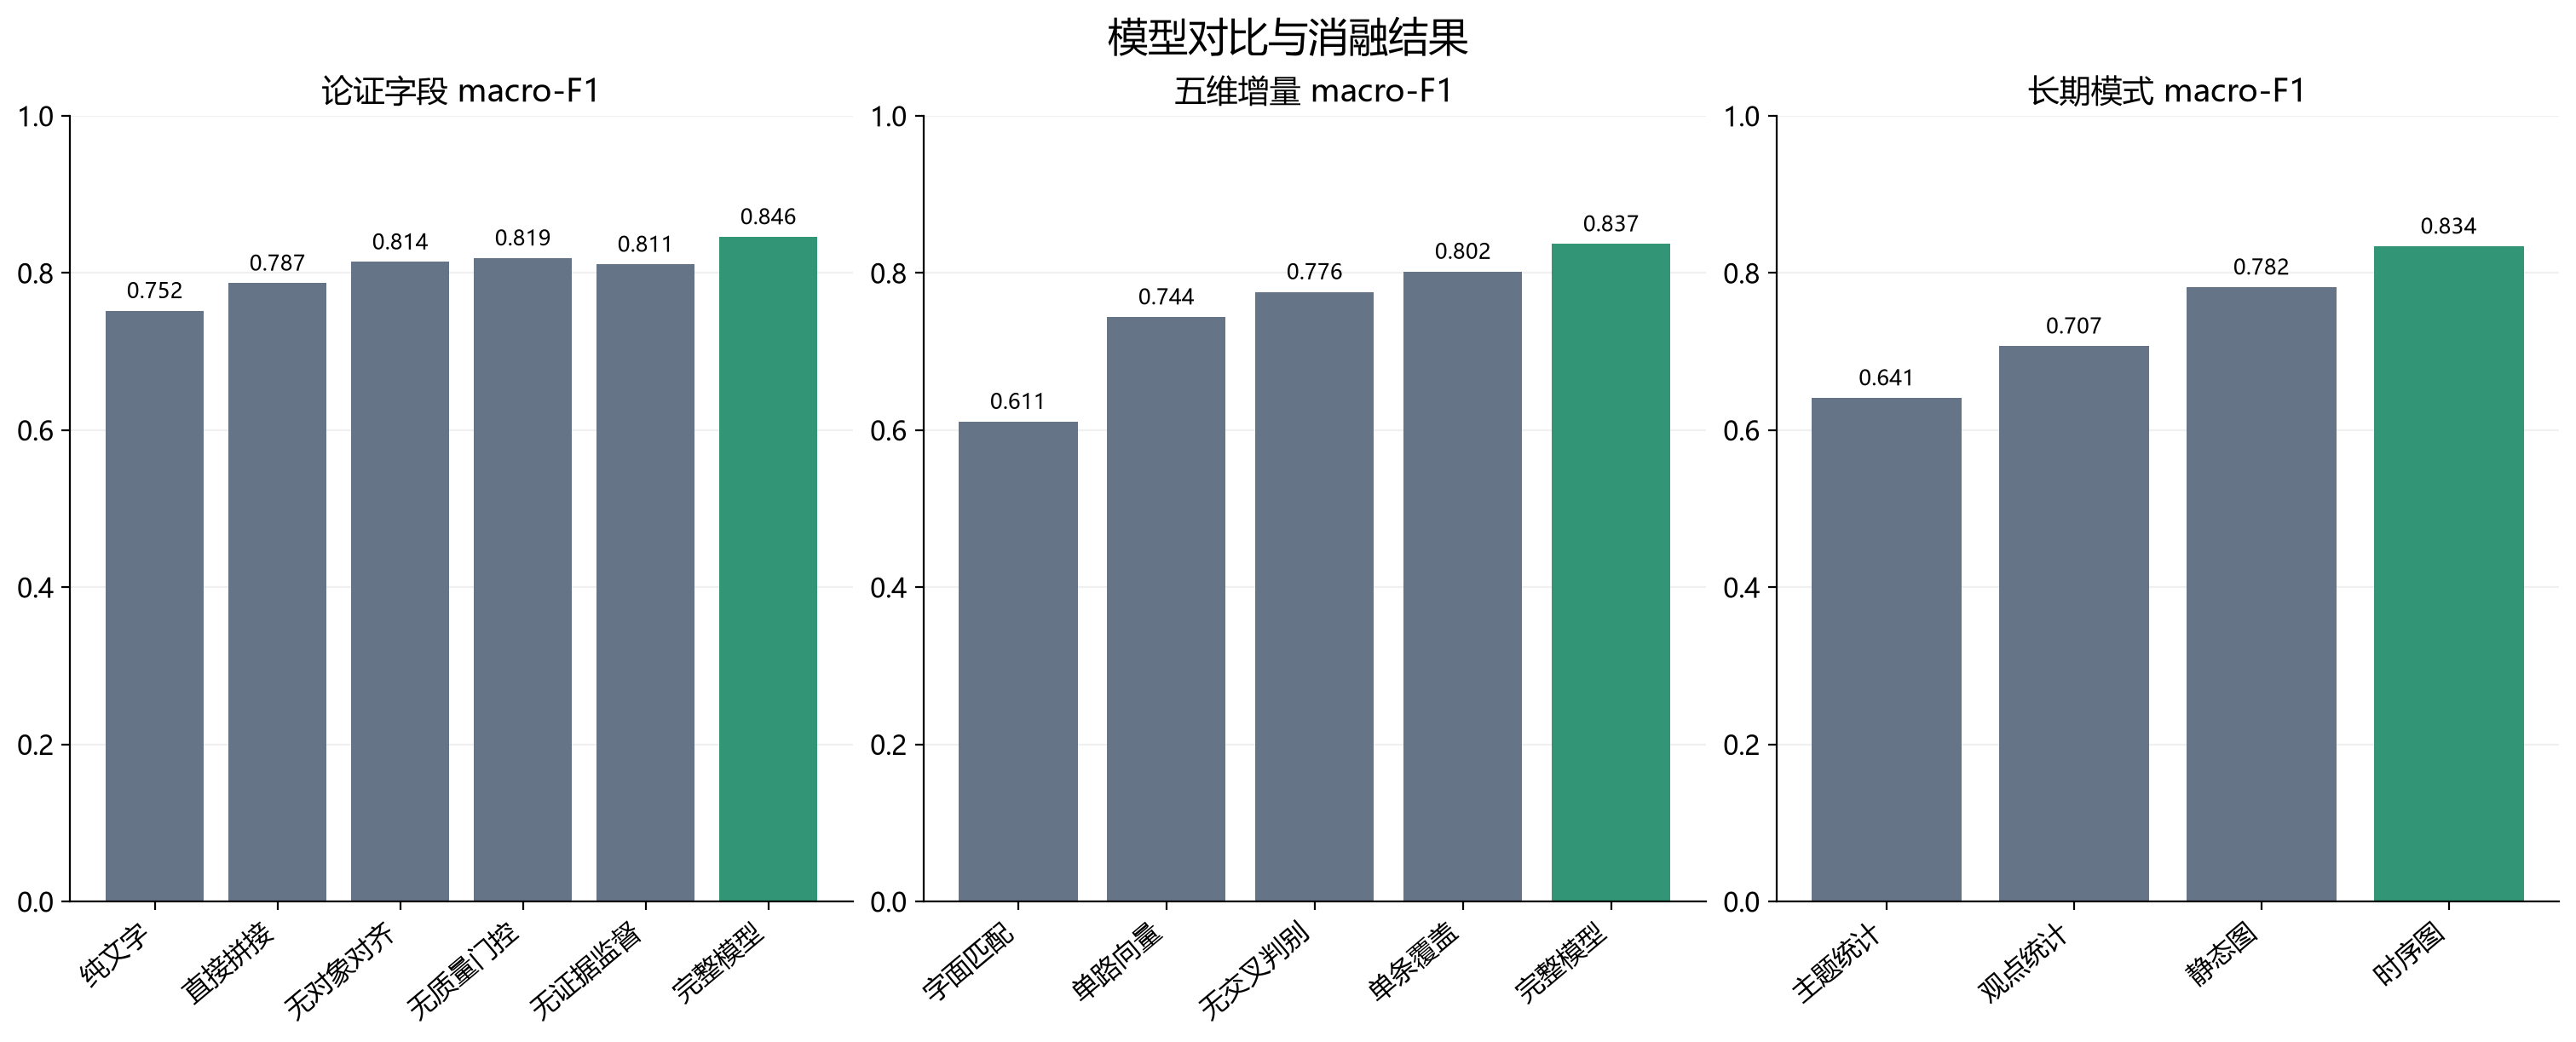
\includegraphics[width=\linewidth,height=0.66\textheight,keepaspectratio]{figures/chapter3/图3-4.png}
\caption{模型对比与消融结果}\label{fig:3-4}
\end{figure}

\subsection{时序论证图与长期接触模式分析}\label{section:3.6}

\subsubsection{对照设置及校准}\label{section:3.6.1}

长期评价采用主题统计、观点统计、静态图特征和带关系消息、时间编码与 GRU 记忆的时序论证图四种方法。测试标签覆盖持续低增量重复、正常专题学习、同源转载、不同立场接触和观察不足。误报率专门在正常专题学习窗口上计算，缺失窗口不作为低风险负例。

\begin{longtable}[]{@{}
  >{\RaggedRight\arraybackslash}p{(\linewidth - 8\tabcolsep) * \real{0.1800}}
  >{\RaggedRight\arraybackslash}p{(\linewidth - 8\tabcolsep) * \real{0.2000}}
  >{\RaggedRight\arraybackslash}p{(\linewidth - 8\tabcolsep) * \real{0.2000}}
  >{\RaggedRight\arraybackslash}p{(\linewidth - 8\tabcolsep) * \real{0.2200}}
  >{\RaggedRight\arraybackslash}p{(\linewidth - 8\tabcolsep) * \real{0.2000}}@{}}
\caption{长期接触模式对照结果}\label{tab:3-8}\tabularnewline
\toprule\noalign{}
方法 & 用户隔离 macro-F1 & 同用户未来 macro-F1 & 专题学习误报率 & 用户隔离 ECE \\
\midrule\noalign{}
\endfirsthead
\toprule\noalign{}
方法 & 用户隔离 macro-F1 & 同用户未来 macro-F1 & 专题学习误报率 & 用户隔离 ECE \\
\midrule\noalign{}
\endhead
\bottomrule\noalign{}
\endlastfoot
主题集中统计 & 0.641 & 0.662 & 23.8\% & 0.112 \\
观点分布统计 & 0.707 & 0.725 & 18.4\% & 0.086 \\
静态论证图及解释特征 & 0.782 & 0.805 & 10.7\% & 0.061 \\
完整时序论证图 & 0.834 & 0.858 & 6.4\% & 0.034 \\
\end{longtable}

ECE 采用 15 个等频置信桶，按桶内预测准确率与置信均值差的绝对值加权计算；温度校准在验证集完成，测试期不重新拟合。用户隔离 macro-F1 达到 0.80，ECE 低于 0.05；同用户未来结果单独反映早期个体背景的作用，不能替代新用户泛化能力。

在用户隔离协议中，移除历史增量、移除来源关系、移除时间编码与记忆后的 macro-F1 分别为 0.766、0.805 和 0.789，完整模型为 0.834。结果说明持续性和论据复用能够补充观点集中统计，跨平台不意味着来源必然独立，正常专题学习也不等于持续低增量重复。

\subsubsection{观察窗口与解释}\label{section:3.6.2}

3 天、7 天和 14 天窗口在用户隔离协议中的 macro-F1 分别为 0.758、0.812 和 0.834。短窗口能迅速定位集中浏览，但更容易混淆阶段性任务与持续重复；长窗口提供较稳定的历史依据，同时提高缺失记录管理要求。系统对有效覆盖不足的窗口输出观察不足状态，而不是依据低数据量生成确定风险分数。

面向用户的解释展示观点集中、低增量重复、旧论据复用、来源关系与持续天数，并连接相关作品和原文。模型估计是接触模式的校准概率，不是``认知受影响程度''的直接测量。专题学习误报仍有 6.4\%，因此报告结合用户阅读目的与阶段性任务说明，不采用单次高分强制干预。

\subsection{情绪诱因、角色与个人反馈评价}\label{section:3.7}

情绪模型围绕候选对矩阵、行列交互和角色链接开展评价；认知评价分支保留适用性与五级强度，生活处境和表达方式使用相应标签。个人反应校准仅使用自愿反馈，内容表达结果与自报结果分开存储和展示。

\begin{longtable}[]{@{}
  >{\RaggedRight\arraybackslash}p{(\linewidth - 8\tabcolsep) * \real{0.1800}}
  >{\RaggedRight\arraybackslash}p{(\linewidth - 8\tabcolsep) * \real{0.2000}}
  >{\RaggedRight\arraybackslash}p{(\linewidth - 8\tabcolsep) * \real{0.2000}}
  >{\RaggedRight\arraybackslash}p{(\linewidth - 8\tabcolsep) * \real{0.2200}}
  >{\RaggedRight\arraybackslash}p{(\linewidth - 8\tabcolsep) * \real{0.2000}}@{}}
\caption{情绪联合模型评价}\label{tab:3-9}\tabularnewline
\toprule\noalign{}
方法 & 情绪---原因配对 F1 & 角色跨度 F1 & 归属准确率 & 认知评价等级 MAE \\
\midrule\noalign{}
\endfirsthead
\toprule\noalign{}
方法 & 情绪---原因配对 F1 & 角色跨度 F1 & 归属准确率 & 认知评价等级 MAE \\
\midrule\noalign{}
\endhead
\bottomrule\noalign{}
\endlastfoot
共享编码、独立配对 & 0.704 & 0.731 & 0.827 & 0.83 \\
二维交互、不使用角色链接 & 0.757 & 0.768 & 0.866 & 0.72 \\
移除认知评价条件化 & 0.774 & 0.807 & 0.900 & 0.69 \\
完整联合模型 & 0.802 & 0.829 & 0.923 & 0.58 \\
\end{longtable}

完整模型配对 F1 超过 0.75。认知评价适用性 F1 为 0.871，生活处境 macro-F1 为 0.816，表达方式 macro-F1 为 0.834；等级 MAE 仅在维度适用且具备金标的样本上计算，未提及状态不编码为最低强度。隐含诱因、多持有者及讽刺表达仍产生错误，空诱因节点保留为未定位而不补造原因。

参与者回顾任务共安排每人每天 1 次、2,800 次，收到 2,240 次反馈，回应率 80.0\%，其中 2,100 次具备完整有效标签、140 次字段不完整，其余 560 次未回应。缺失反馈不作为``无焦虑''。在用户隔离测试的 360 次有效反馈上，内容表达直接映射个人反应的等级 MAE 为 0.92，经过独立校准为 0.74；时间隔离测试使用 420 次有效反馈，早期反馈个体适配后的 MAE 为 0.62。两个协议样本来自不同划分，指标不能拼接为总体效果。

该结果衡量模型与参与者自报的一致性，不是临床效度，也不证明浏览内容导致某种情绪。反馈可以撤回，撤回后重建受影响的校准状态和报告。

\subsection{异步处理与系统性能}\label{section:3.8}

\subsubsection{负载与统计范围}\label{section:3.8.1}

基础负载为 30 台逻辑在线设备，每台每分钟 20 个新事件，合计 10 个事件/秒。每轮预热 10 分钟后连续运行 60 分钟，共 36,000 个事件，重复 5 轮共 180,000 个事件。采用固定数据集片段回放，回放次数只用于负载测量，不增加自然作品样本规模。端到端时延从客户端发送起点测量，服务器排队与计算分别记录；公网不确定波动不纳入受控网络下的服务容量结论。

每轮测量接收确认、首个可用语义结果、完整分析、报告更新、GPU 利用率与各阶段队列。P95 先在每轮事件上计算，表中报告 5 轮 P95 的均值；吞吐按完成数量除以测量时长计算。模型完成时延包含队列、OCR/ASR 及后续历史和图更新，不能以快速接收确认替代。

\begin{longtable}[]{@{}
  >{\RaggedRight\arraybackslash}p{(\linewidth - 6\tabcolsep) * \real{0.2500}}
  >{\RaggedRight\arraybackslash}p{(\linewidth - 6\tabcolsep) * \real{0.2500}}
  >{\RaggedRight\arraybackslash}p{(\linewidth - 6\tabcolsep) * \real{0.2500}}
  >{\RaggedRight\arraybackslash}p{(\linewidth - 6\tabcolsep) * \real{0.2500}}@{}}
\caption{10 事件/秒基础负载结果}\label{tab:3-10}\tabularnewline
\toprule\noalign{}
指标 & 测量值 & 内部验收依据或解释 & 状态 \\
\midrule\noalign{}
\endfirsthead
\toprule\noalign{}
指标 & 测量值 & 内部验收依据或解释 & 状态 \\
\midrule\noalign{}
\endhead
\bottomrule\noalign{}
\endlastfoot
接收确认 P50/P95 & 118/286 毫秒 & P95≤500 毫秒，使快速浏览先得到记录状态 & 达标 \\
首个可用语义结果 P50/P95 & 0.91/2.18 秒 & 阶段结果与浏览并行，不阻塞客户端 & 通过 \\
完整模型分析 P50/P95 & 3.82/8.74 秒 & 独立报告精细理解尾延迟 & 通过 \\
完成后报告更新 P95 & 420 毫秒 & 统计更新不等待下一次浏览 & 通过 \\
事件级最终完成吞吐 & 10.00 事件/秒 & 到达与长期完成相匹配 & 达标 \\
待完成队列 P95 & 72 个事件 & 包含正在处理及排队的多阶段事件 & 通过 \\
每轮最后 10 分钟净积压变化 & −3 至+4 个事件 & 无持续增长，有限波动 & 达标 \\
单 GPU 平均利用率 & 72\% & 体现基础负载下的资源余量 & 通过 \\
\end{longtable}

各阶段饱和能力分别为初步理解 24、OCR 13、ASR 4.1、精细理解 5.4、历史比较 19、图更新 42 个任务/秒；相应基础到达率为 10、5、2、3、10、10 个任务/秒。OCR/ASR 等能力按各自任务定义测量，不能直接相加为系统作品吞吐。

\begin{figure}[htbp]
\centering
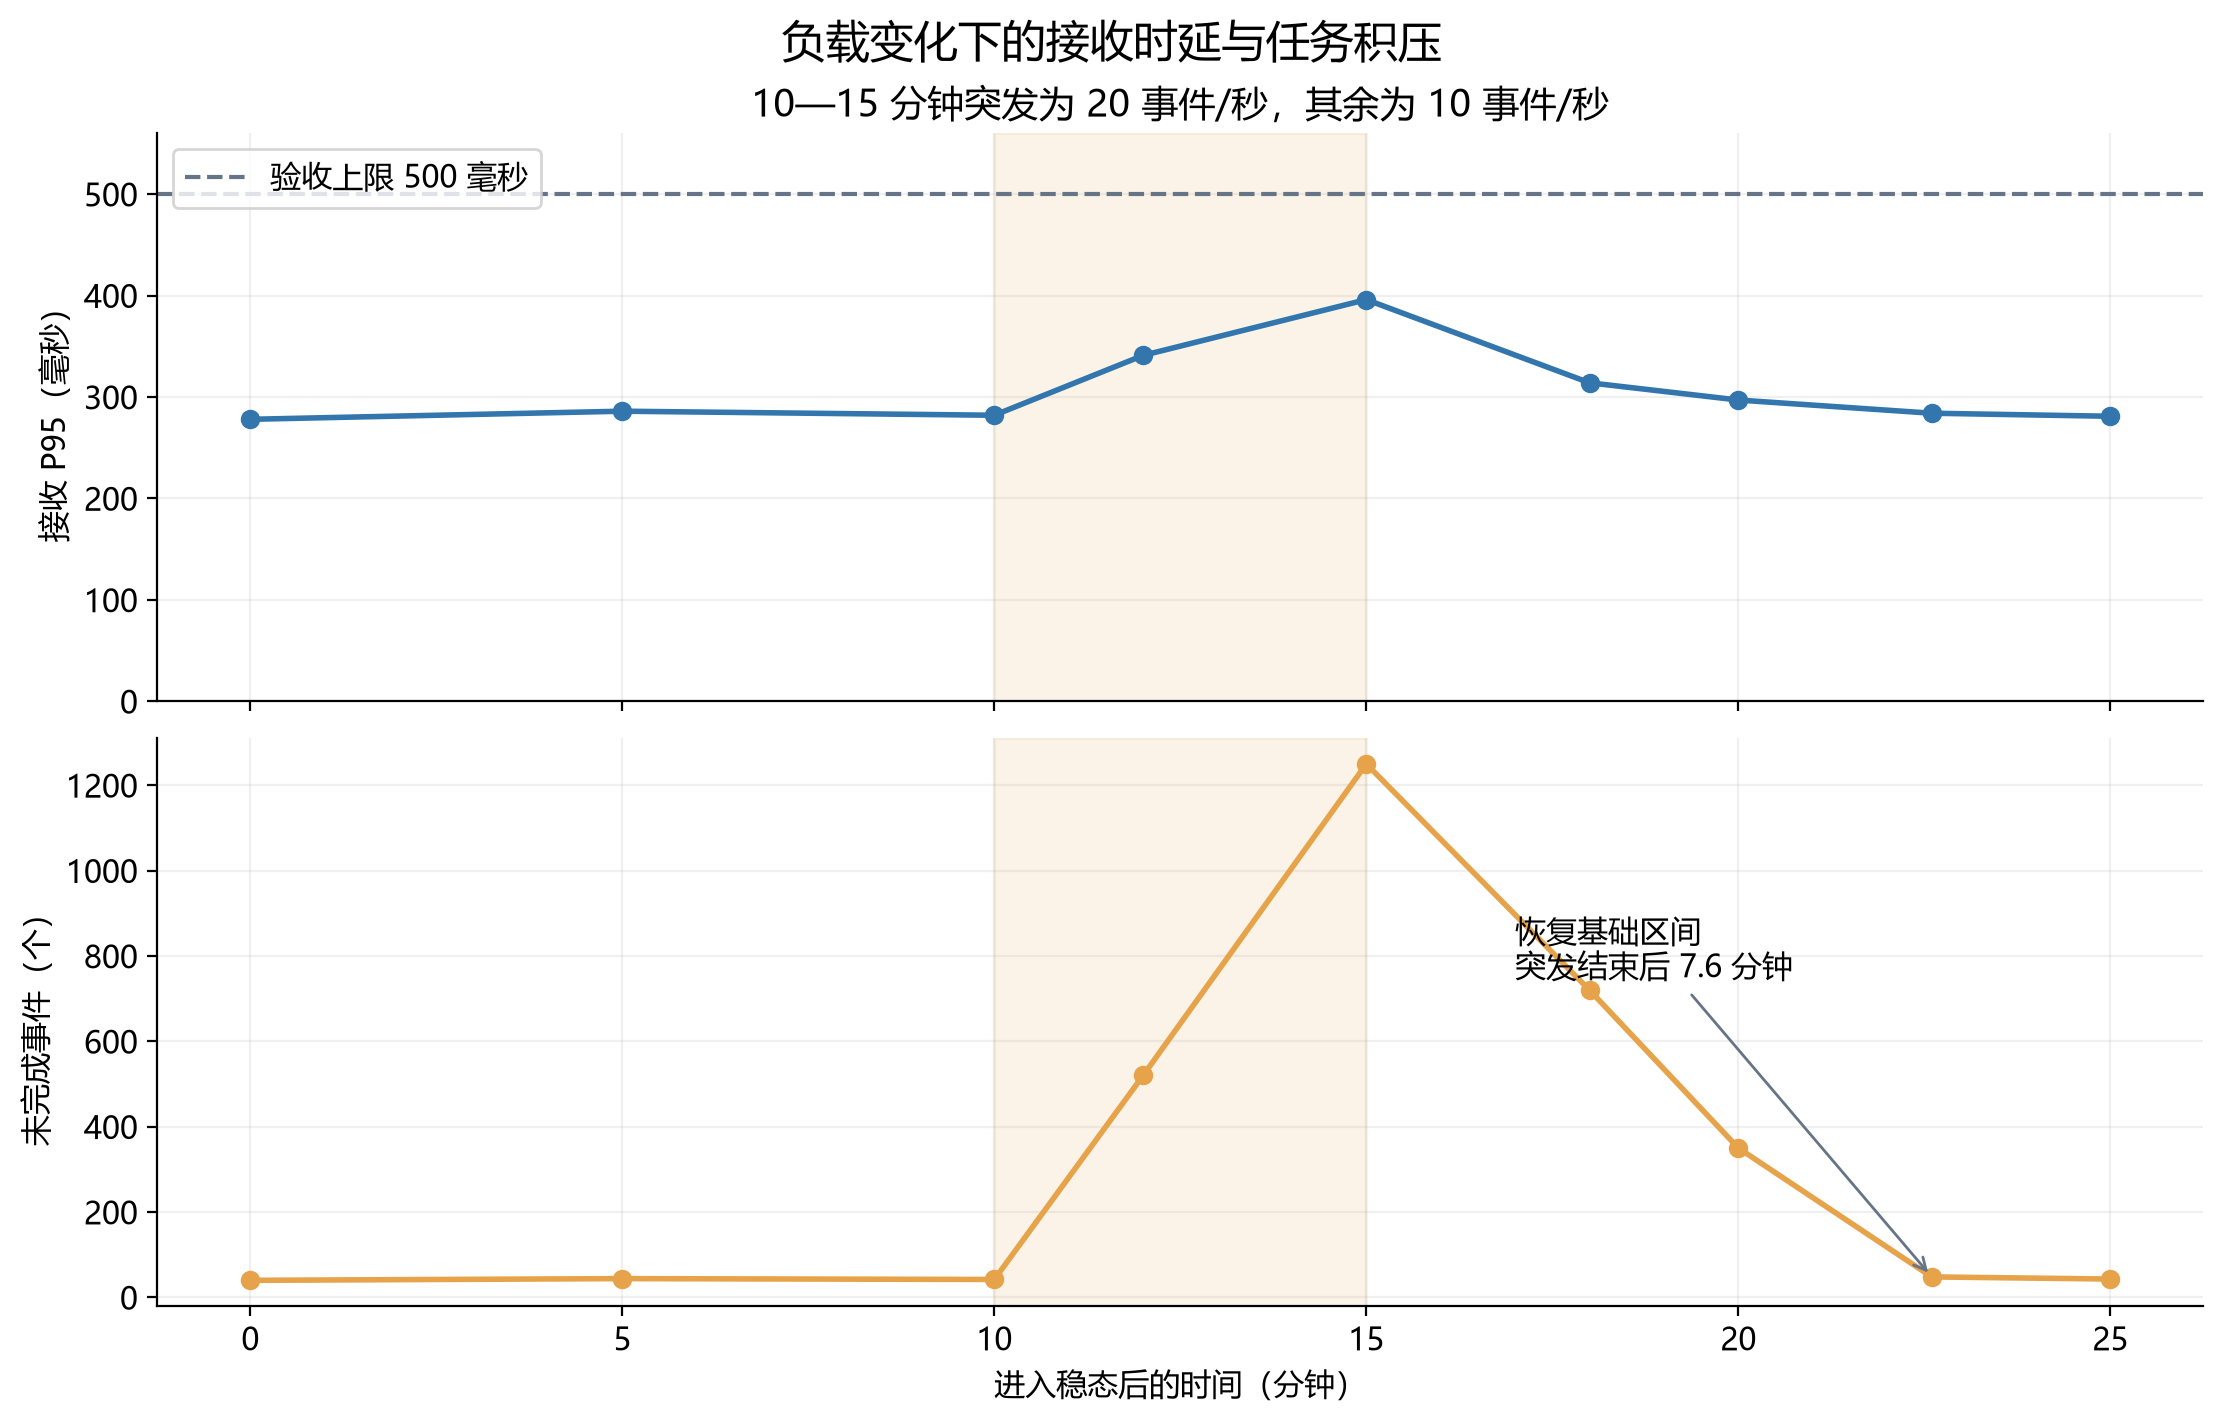
\includegraphics[width=\linewidth,height=0.66\textheight,keepaspectratio]{figures/chapter3/图3-5.png}
\caption{负载变化下的接收时延与任务积压}\label{fig:3-5}
\end{figure}

\begin{longtable}[]{@{}
  >{\RaggedRight\arraybackslash}p{(\linewidth - 6\tabcolsep) * \real{0.2500}}
  >{\RaggedRight\arraybackslash}p{(\linewidth - 6\tabcolsep) * \real{0.2500}}
  >{\RaggedRight\arraybackslash}p{(\linewidth - 6\tabcolsep) * \real{0.2500}}
  >{\RaggedRight\arraybackslash}p{(\linewidth - 6\tabcolsep) * \real{0.2500}}@{}}
\caption{突发负载及队列恢复过程}\label{tab:3-11}\tabularnewline
\toprule\noalign{}
时间（分钟） & 输入事件/秒 & 最近一分钟接收 P95（毫秒） & 未完成事件 \\
\midrule\noalign{}
\endfirsthead
\toprule\noalign{}
时间（分钟） & 输入事件/秒 & 最近一分钟接收 P95（毫秒） & 未完成事件 \\
\midrule\noalign{}
\endhead
\bottomrule\noalign{}
\endlastfoot
0 & 10 & 278 & 40 \\
5 & 10 & 286 & 44 \\
10，突发前 & 10 & 282 & 42 \\
12 & 20 & 341 & 520 \\
15，突发结束前 & 20 & 396 & 1,250 \\
18 & 10 & 314 & 720 \\
20 & 10 & 297 & 350 \\
22.6 & 10 & 284 & 48 \\
25 & 10 & 281 & 43 \\
\end{longtable}

图~\ref{fig:3-5}显示，突发负载结束后 7.6 分钟，未完成任务数量恢复至基础负载区间。曲线中的瞬时积压量与 5 轮基础负载测试的队列 P95（72）分别统计；较短的接收时延不代表精细分析无需排队。

\subsubsection{突发、恢复与端侧开销}\label{section:3.8.2}

持续 5 分钟输入 20 事件/秒时，资源受限阶段积压增加；恢复 10 事件/秒后，队列在 7.6 分钟内回到基础区间。系统未丢弃已经确认接收的事件，低质量或重复片段的跳过均记录原因。断网 60 秒后的端侧重传不重复计数，服务器重启后的未完成任务根据阶段与版本重入队列，恢复不依赖明文日志。

真机连续观察 30 分钟时，相对同内容浏览基线，新增电量消耗为 2.1 个百分点，设备表面温升增量为 1.8 ℃，前台丢帧率由 2.4\%升至 3.2\%。测试固定屏幕亮度、刷新率和网络，采用同设备配对实验，不能把两款不同手机的电量差作为采集服务开销。授权上传量在该混合负载下平均为 0.62 MB/事件，视频片段贡献较高，用户可以关闭媒体采集以减少流量，但报告同步降低相应观察覆盖。

\subsection{可验证机密计算与安全测试}\label{section:3.9}

\subsubsection{威胁模型及用例分类}\label{section:3.9.1}

外部服务域的攻击能力包括读取外部存储、修改报文、替换镜像、恢复旧快照和干扰消息顺序。客户端密钥管理、硬件隔离、证明信任根及获准服务构成可信计算基；客户端最新检查点有效保存是历史新鲜度判断的前提。终端完全失陷、未知硬件漏洞、访问时序完全隐藏和拒绝服务消除不属于已证明性质。

120 个场景按 12 类组织，每类 10 个参数化场景。Mock 模式运行全部状态机用例；其中 90 个证明、链路与状态场景另在真实 CPU 机密环境重复，60 个包含 GPU 设备与通信边界的相关场景再于 GPU 机密环境重复。场景重复执行不新增场景种类，也不以 Mock 结果替代硬件证明。

\begin{longtable}[]{@{}
  >{\RaggedRight\arraybackslash}p{(\linewidth - 6\tabcolsep) * \real{0.1600}}
  >{\RaggedRight\arraybackslash}p{(\linewidth - 6\tabcolsep) * \real{0.2800}}
  >{\RaggedRight\arraybackslash}p{(\linewidth - 6\tabcolsep) * \real{0.2800}}
  >{\RaggedRight\arraybackslash}p{(\linewidth - 6\tabcolsep) * \real{0.2800}}@{}}
\caption{安全测试结果与证明范围}\label{tab:3-12}\tabularnewline
\toprule\noalign{}
场景类型 & 注入输入或步骤 & 预期结果 & 结果及证明范围 \\
\midrule\noalign{}
\endfirsthead
\toprule\noalign{}
场景类型 & 注入输入或步骤 & 预期结果 & 结果及证明范围 \\
\midrule\noalign{}
\endhead
\bottomrule\noalign{}
\endlastfoot
正常握手 & 正确挑战、公钥、清单与证明链 & 建链、密钥确认、授权后执行 & 10/10 通过；证明允许流程可用 \\
挑战重用 & 使用旧挑战或重放证明 & 放行谓词拒绝，存储密钥不释放 & 10/10 拒绝；验证本次会话新鲜度 \\
公钥替换 & 替换任一临时公钥 & 转录绑定或密钥确认失败 & 10/10 拒绝；验证端点绑定 \\
测量与清单不符 & 修改镜像、模型摘要、工具权限或调试策略 & 策略不匹配，不进入授权阶段 & 10/10 拒绝；依赖加载器正确校验 \\
密文与对象篡改 & 修改密文、关联数据、对象结构版本 & AEAD 或对象校验失败 & 10/10 拒绝；不证明语义内容真实 \\
序号重放 & 旧 seq 报文再次发送 & 重放拒绝，事件状态不重复推进 & 10/10 拒绝；业务重试另用幂等标识 \\
用途与方向混用 & 交换上传/下载或数据/控制密钥上下文 & 认证失败 & 10/10 拒绝；验证四类密钥分离 \\
旧快照恢复 & 宿主机提供旧版本及旧对象根 & 与最新客户端锚点不符，转入重同步 & 10/10 拒绝；要求最新锚点未丢失 \\
确认前后掉线 & 在两阶段提交各边界切断连接 & 待提交不冒充已提交，凭锚点续传 & 10/10 状态一致；不承诺网络可用性 \\
越权与缓存串用 & 用户交叉请求、标识复用及会话切换 & 拒绝跨用户对象与图记忆访问 & 10/10 拒绝；检查内存、索引与队列 \\
删除及依赖重放 & 删除旧事件、论据或反馈 & 清理依赖闭包，重建报告与记忆 & 10/10 通过；密码销毁另核验密钥副本 \\
授权撤回及 GPU 边界 & 会话撤权、GPU 证明无效或链路不合策略 & 停止对应任务、清理缓存或禁止 GPU 执行 & 10/10 通过预期拒绝/清理行为 \\
\end{longtable}

恶意页面中的指令性文字只进入分析数据层。附加 200 条指令注入探针覆盖诱导外联、修改工具权限与跨用户查询，均未产生未授权工具调用；该结果只覆盖探针集合，不能推导模型对任何新型注入都免疫。

\subsubsection{历史提交、删除与可追溯性}\label{section:3.9.2}

客户端检查点包含用户标识、密钥代次、提交版本、Merkle 根及前驱摘要。服务器准备状态后回读对象，客户端原子保存检查点再确认；恢复先核对根和最新确认版本，再在可信边界内解密。客户端已保存而服务端未收到确认的事务能够凭检查点完成；尚未保存的候选版本保持待提交。恢复用例未出现旧快照被误当作最新已确认状态。

删除沿依赖闭包移除转写、向量、关系和缓存，并按固定模型版本从有效检查点重放保留事件。日报、历史比较和时序记忆同步修订，多来源摘要按保留材料重建。涉及密码学销毁时回收对应密钥代次及受管理备份，已经导出到用户终端或第三方位置的报告不宣称能够被远程撤回。

日志检查未发现原文、提示模板输入、向量或报告明文落入外部日志。宿主机可见任务大小与访问时间等元数据仍存在，合并请求及分级填充降低粒度但不实现完全不可观察。硬件与客体运行时均属于需要持续维护的安全前提，证明有效不等于分析结论必然正确。

\subsubsection{机密执行开销}\label{section:3.9.3}

在同一 NCC40ads H100 v5 硬件、同一模型和同一回放序列上比较常规与机密模式，不采用跨云 A10G 与 H100 的时间差。完整分析平均时延分别为 3.40 秒与 3.78 秒，增量为 11.18\%；接收确认 P95 由 254 毫秒增至 286 毫秒，增量为 12.60\%。单次会话证明与建链 P95 为 1.34 秒，不计入已建链事件接收时延；增量状态提交 P95 为 168 毫秒，1 GB 历史恢复 P95 为 2.84 秒。

开销来自证明、受保护传输、加密对象与检查点提交。会话复用摊薄证明成本，但会话过期、版本切换及重启均重新证明。上述相对开销只适用于本章规定输入和硬件，不能外推为全部模型与实例的固定开销。

\begin{figure}[htbp]
\centering
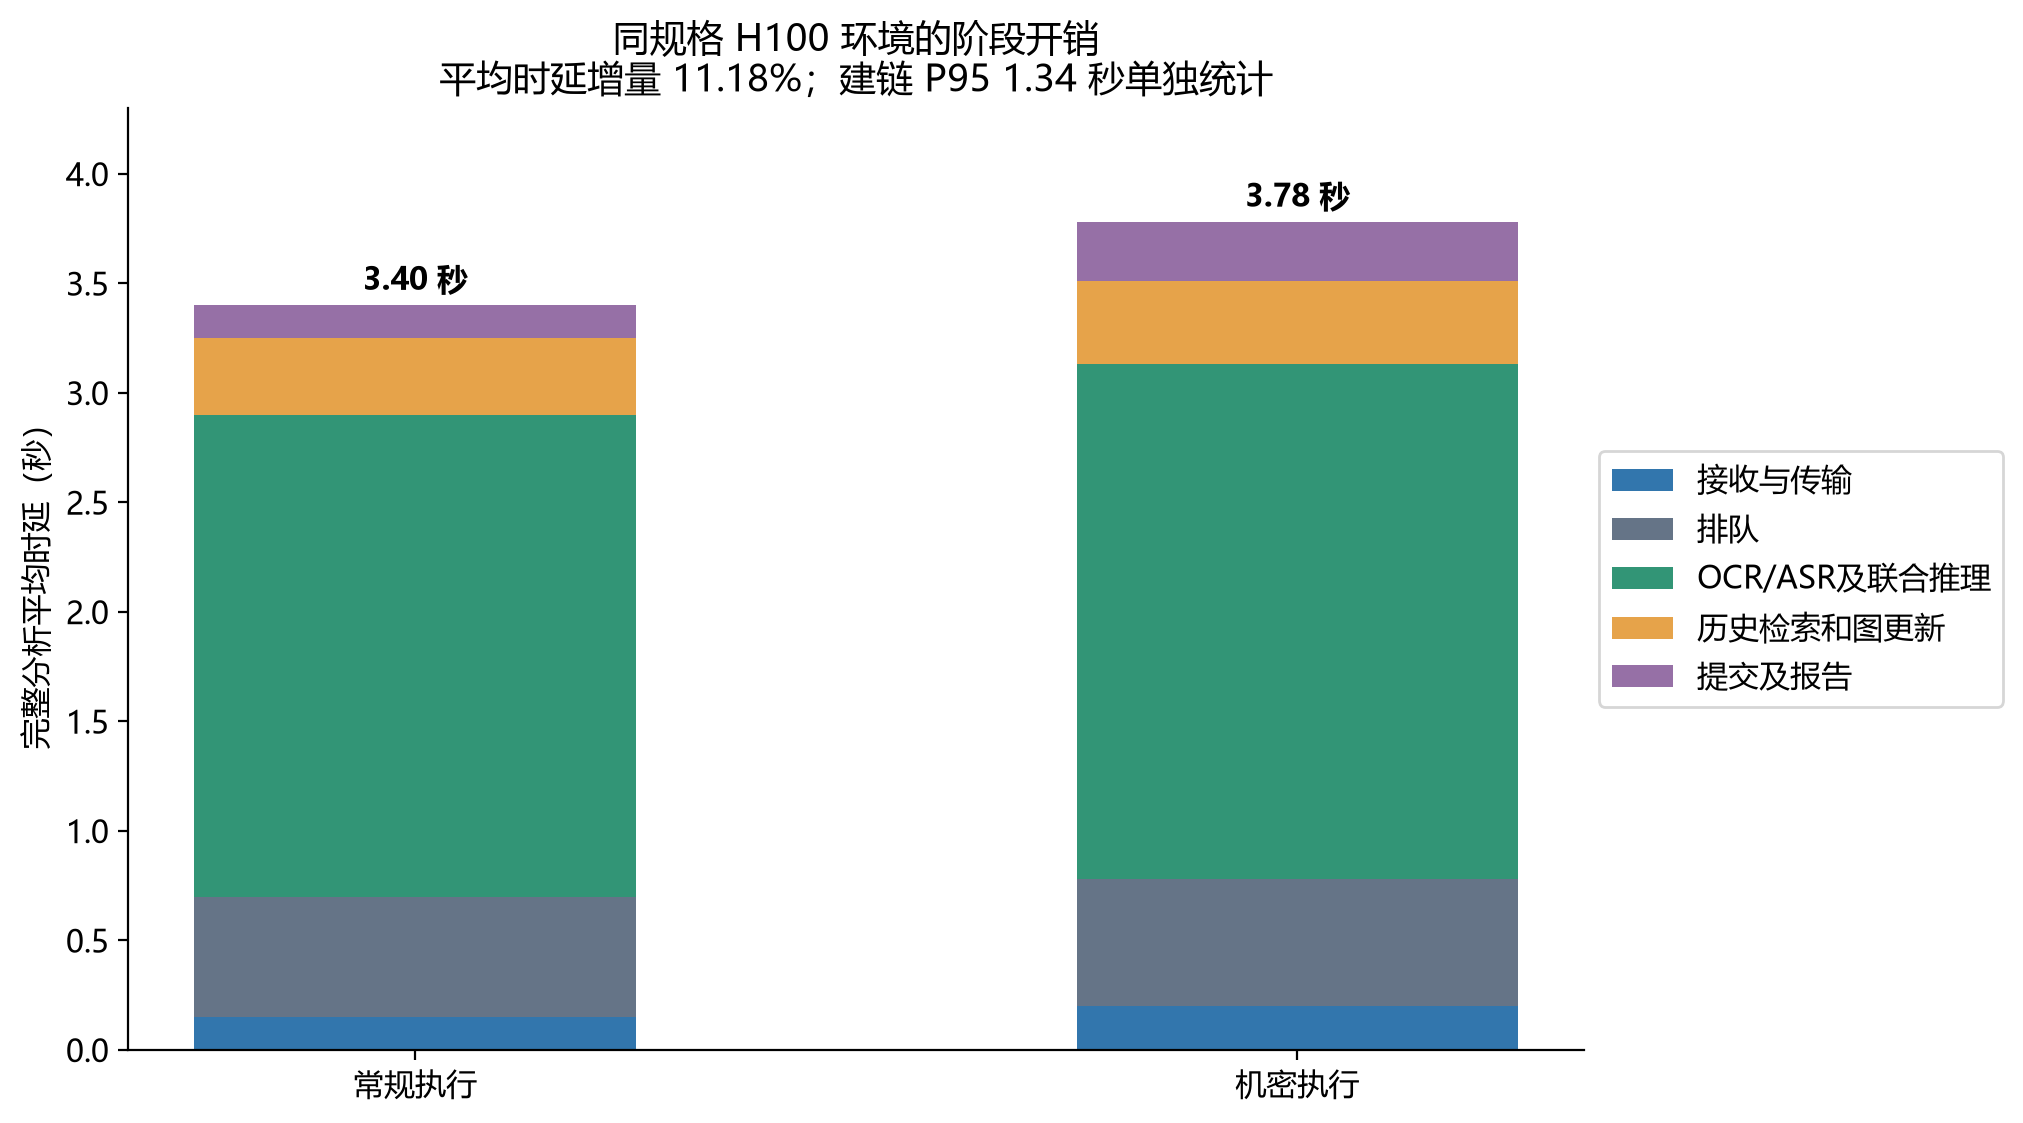
\includegraphics[width=\linewidth,height=0.66\textheight,keepaspectratio]{figures/chapter3/图3-6.png}
\caption{常规与机密执行的阶段开销}\label{fig:3-6}
\end{figure}

\subsection{复赛新增协同API路径的独立验收范围}
新增协同API路径的测试与前述初赛实验分别记录。协议回归涵盖会话签名、载荷认证、历史版本和哈希匹配、失败不推进状态及重试处理；这些离线用例不能替代硬件远程证明或商业模型准确率评价。Room v10新增按日期及议题组织的物化统计，并以事件贡献和事实身份索引维护删除、重分析及跨日去重。预热后的摘要查询、首次回填和包含原文排版的完整PDF生成必须分别计时，不能用摘要查询时间宣称完整报告生成低于15毫秒。

商业API与本地轻量化基准的事实合并F1、情绪引导F1、误报率及端到端P50/P95，需要在相同保留测试集、固定模型版本与网络条件下重新测量。本轮代码与离线协议验收不提供这些新实验结果，故不填入预设的提升幅度或亚秒延迟。新版Android信息盲区、原文对照及管理端攻防截图仅在实际运行后采集，不以示意图冒充实机结果。详细执行记录见仓库\texttt{BUILD\_VALIDATION.md}及\texttt{docs/R3\_FINAL\_ITERATION\_PLAN.md}。

\subsection{验收依据、结果分析与章节小结}\label{section:3.10}

\subsubsection{内部验收标准及达标情况}\label{section:3.10.1}

\begin{longtable}[]{@{}
  >{\RaggedRight\arraybackslash}p{(\linewidth - 8\tabcolsep) * \real{0.1600}}
  >{\RaggedRight\arraybackslash}p{(\linewidth - 8\tabcolsep) * \real{0.2500}}
  >{\RaggedRight\arraybackslash}p{(\linewidth - 8\tabcolsep) * \real{0.2500}}
  >{\RaggedRight\arraybackslash}p{(\linewidth - 8\tabcolsep) * \real{0.2500}}
  >{\RaggedRight\arraybackslash}p{(\linewidth - 8\tabcolsep) * \real{0.0900}}@{}}
\caption{核心验收结果}\label{tab:3-13}\tabularnewline
\toprule\noalign{}
项目 & 内部阈值 & 本章结果 & 阈值设置依据 & 结论 \\
\midrule\noalign{}
\endfirsthead
\toprule\noalign{}
项目 & 内部阈值 & 本章结果 & 阈值设置依据 & 结论 \\
\midrule\noalign{}
\endhead
\bottomrule\noalign{}
\endlastfoot
作品计数 & P、R 均≥95\% & 98.48\%、97.81\% & 同时限制误拆分和漏记，避免只追求单侧指标 & 达标 \\
可见停留 & MAE≤2 秒 & 1.12 秒 & 降低快速切换时区间误差，区别实际阅读估计 & 达标 \\
幂等、修订、隔离 & 指定工程用例全部通过 & 无违反预期的状态贡献 & 重复上传和越权不应依靠概率容忍 & 通过 \\
论证字段 & macro-F1≥0.80 & 0.846 & 控制小类别退化，支持结构化证据回看 & 达标 \\
主体归属 & 准确率≥0.90 & 0.934 & 限制引用者与被引述者混淆 & 达标 \\
历史召回 & Recall@50≥0.90 & 0.941 & 降低漏检旧依据导致的虚假新增 & 达标 \\
五维增量 & macro-F1≥0.80 & 0.837 & 分开检查事实、论据、条件、解释与行动 & 达标 \\
长期模式 & macro-F1≥0.80、ECE≤0.05 & 0.834、0.034 & 平衡模式区分与概率可信程度 & 达标 \\
情绪---原因 & 配对 F1≥0.75 & 0.802 & 考虑跨片段配对难度，避免只输出情绪词 & 达标 \\
安全约束 & 定义的恶意用例全部拒绝 & 全部达到预期拒绝/隔离行为 & 放行前提与认证检查属于硬约束 & 通过 \\
基础容量 & 10 事件/秒；接收 P95≤500 毫秒；积压不持续增长 & 286 毫秒；完成 10.00 事件/秒；队列稳定 & 对应 30 设备快速浏览场景与异步交互 & 达标 \\
\end{longtable}

这些阈值是本项目的内部验收约定，来源于业务约束、漏检后果和交互目标，不是行业统一标准。阈值在查看测试结果之前冻结，不能在测试后通过降低标准得到达标结论。模型仍存在不确定与误差，因此通过验收不意味着所有输入均可分析。

\subsubsection{综合分析}\label{section:3.10.2}

采集层通过作品与事件分离减少重复计数，统计层通过区间并集和修订替换避免时长累加失真。多模态理解将观点组织为具有对象、立场、条件和论据的结构，证据定位与质量门控提高可解释性。历史联合覆盖能够处理旧依据分散在多个作品中的情况，使同观点新论据与低增量重复得到不同结果。

时序论证图相对于主题统计降低正常专题学习的误报，表明持续性、信息增量与来源关系是必要补充；情绪角色和认知评价分支减少内容表达与人物归属混淆。机密计算测试验证了规定威胁模型下的执行主体、通道与历史状态约束，但没有扩大为绝对隐私或模型真实性保证。

剩余改进集中在平台页面结构变化、极快切换、隐含条件、反讽、多主体归属和长尾议题。长期分析还受到观察覆盖和参与者反馈缺失影响。系统通过拒识、覆盖说明、证据回看与用户更正处理这些边界，报告的用途是支持个人审视信息环境，而不是替用户作出认同判断或心理诊断。

\subsubsection{本章小结}\label{section:3.10.3}

本章建立了与技术路线对应的分层测试体系，完成作品采集、阅读估计、跨模态论证、个人历史增量、时序图、情绪建模、异步处理和可信执行评价。核心模型指标达到内部标准，基础负载下接收和处理保持稳定，协议与状态用例满足规定约束。实验同时保留误差、拒识与未知范围，使工程达标、语义效果和安全边界分别得到解释。
